\section{Code Quality}
	RaceTrack is being developed using the leading cloud-based solution for continuous analysis of code quality, reliability, and security \textbf{SonarCloud}. Not only does \textbf{SonarCloud} automatically detect bugs, vulnerabilities, code smells and, other issues, it also elevates the team's coding quality to a new standard. 
	\begin{figure}[H]
		\centering
		
\includegraphics[width=8cm,keepaspectratio,center]{img/Implementation_SonarCloud_Shields.png}
		\caption{SonarCloud Summary for RaceTrack}
	\end{figure}
	RaceTrack currently maintains the highest Reliability Rating \textcolor{ForestGreen}{A}, the highest Security Rating \textcolor{ForestGreen}{A} and an outstanding Test Coverage of \textcolor{ForestGreen}{81.5\%}, and all of that still in the Beta Phase, with only room for further improvement.
	\begin{figure}[H]
		\centering
		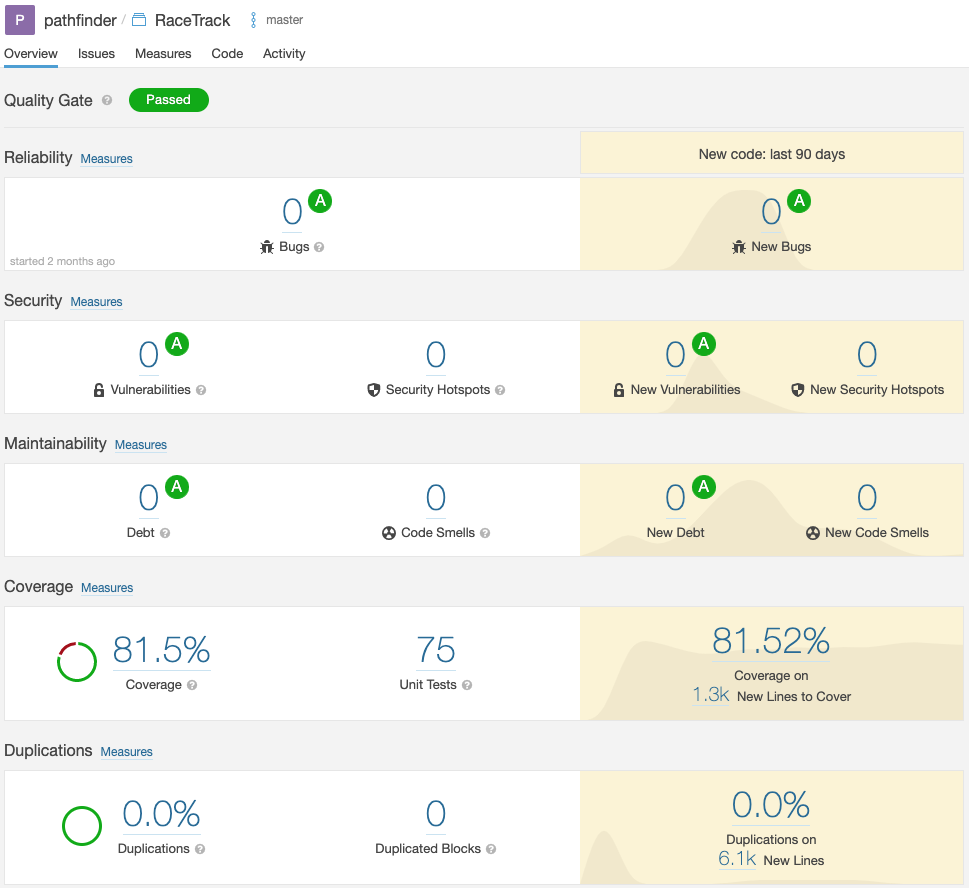
\includegraphics[width=16cm,keepaspectratio,center]{img/Implementation_SonarCloud_Dashboard.png}
		\caption{SonarCloud Dashboard for RaceTrack}
	\end{figure}
	In the current build version of RaceTrack, there are also no \textit{code smells} (code that is confusing or difficult to maintain) present.
